\part{Jeux et récréations}

\section{SudoMaths, en \TikZ}\label{sudomaths}

\subsection{Introduction}

\begin{tipblock}
L'idée est de \textit{proposer} un environnement \TikZ, une commande permettant de tracer des grilles de SudoMaths.

L'environnement créé, lié à \TikZ, trace la grille de SudoMaths (avec les blocs démarqués), et peut la remplir avec une liste d'éléments.
\end{tipblock}

\begin{PresCodeTexPL}{listing only}
%grille classique non remplie, avec légendes H/V, {} nécessaires pour préciser que les cases seront "vides"
\SudoMaths{}
\end{PresCodeTexPL}

\begin{PresCodePL}{}
\SudoMaths{}
\end{PresCodePL}

\begin{noteblock}
La commande \ctex{SudoMaths} crée donc la grille (remplie ou non), dans un environnement \TikZ, c'est \textit{c'est tout} ! 

\smallskip

On peut également utiliser l'\textit{environnement} \ctex{EnvSudoMaths} dans lequel on peut rajouter du code \TikZ{} !
\end{noteblock}

\begin{PresCodeTexPL}{listing only}
%grille "toute seule"
\SudoMaths[clés]{liste}

%grille avec ajout de code
\begin{EnvSudoMaths}[clés]{grille}
	%commandes tikz
\end{EnvSudoMaths}
\end{PresCodeTexPL}

\pagebreak

\subsection{Clés et options}

\begin{cautionblock}
Quelques \Cle{clés} sont disponibles pour cette commande :

\begin{itemize}
	\item la clé \Cle{Epaisseurg} pour gérer l'épaisseur des traits épais ; \hfill~défaut \Cle{1.5pt}
	\item la clé \Cle{Epaisseur} pour gérer l'épaisseur des traits fins ; \hfill~défaut \Cle{0.5pt}
	\item la clé \Cle{Unite} qui est l'unité graphique de la figure ; \hfill~défaut \Cle{1cm}
	\item la clé \Cle{CouleurCase} pour la couleur (éventuelles) des cases ; \hfill~défaut \Cle{cyan!50}
	\item la clé \Cle{CouleurTexte} pour gérer la couleur du label des cases ; \hfill~défaut \Cle{blue}
	\item la clé \Cle{NbCol} qui est le nombre de colonnes ; \hfill~défaut \Cle{9}
	\item la clé \Cle{NbSubCol} qui est le nombre de sous-colonnes ; \hfill~défaut \Cle{3}
	\item la clé \Cle{NbLig} qui est le nombre de lignes ; \hfill~défaut \Cle{9}
	\item la clé \Cle{NbSubLig} qui est le nombre de sous-colonnes ; \hfill~défaut \Cle{3}
	\item la clé \Cle{Police} qui formatte le label des cases ; \hfill~défaut \Cle{\textbackslash{}normalfont\textbackslash{}normalsize}
	\item le booléen \Cle{Legendes} qui affiche ou non les légendes (H et V) des cases ; \hfill~défaut \Cle{true}
	\item la clé \Cle{PoliceLeg} qui formatte le label des légendes ; \hfill~défaut \Cle{\textbackslash{}normalfont\textbackslash{}normalsize}
	\item la clé \Cle{ListeLegV} qui est la liste de la légende verticale ; \hfill~défaut \Cle{ABCD...WXYZ}
	\item la clé \Cle{ListeLegH} qui est la liste de la légende horizontale ; \hfill~défaut \Cle{abcd...wxyz}
	\item la clé \Cle{DecalLegende} qui est le décalage de la légende par rapport à la grille. \hfill~défaut \Cle{0.45}
\end{itemize}
\vspace*{-\baselineskip}\leavevmode
\end{cautionblock}

\begin{noteblock}
La liste éventuelle des éléments à rentrer dans le tableau est traitée par le package \ctex{listofitems}, et se présente sous la forme suivante : \ctex{ / / / ... / / § / / / ... / / § ... § / / / ... / / }

\smallskip

Il peut donc être intéressant de \textit{déclarer} la liste au préalable pour simplifier la saisie de la commande !
\end{noteblock}

\begin{noteblock}
La \Cle{CouleurCase} est gérée -- en interne -- par le caractère \ctex{*} qui permet de préciser qu'on veut que la case soit coloriée.
\end{noteblock}

\begin{PresCodeTexPL}{listing only}
%grille 6x6 avec blocs 2x3, avec coloration de cases (présentée sous forme de "cases")
\def\grilleSuMa{%
		(a)* / (b)* /      /      / (c)* / (d)* §%
		(e)* /      /      / (f)* / (g)* / (h)* §%
		     /      / (i)* /      /      / (j)* §%
		     /      / (k)* /      / (l)* / (m)* §%
		(n)* /      / (o)* /      /      / (p)* §%
		     /      /      / (q)* /      /      §%
	}

\SudoMaths[Unite=0.75cm,NbCol=6,NbSubCol=2,NbLig=6,NbSubLig=3,%
	Police=\small\bfseries\ttfamily,CouleurTexte=red,CouleurCase=yellow!50,%
	Legendes=false]{\grilleSuMa}
\end{PresCodeTexPL}

\begin{PresCodeSortiePL}{text only}
\def\grilleSuMa{%
		(a)* / (b)* /      /      / (c)* / (d)* §%
		(e)* /      /      / (f)* / (g)* / (h)* §%
		/      / (i)* /      /      / (j)* §%
		/      / (k)* /      / (l)* / (m)* §%
		(n)* /      / (o)* /      /      / (p)* §%
		/      /      / (q)* /      /      §%
	}

\SudoMaths[Unite=0.75cm,NbCol=6,NbSubCol=2,NbLig=6,NbSubLig=3,Police=\small\bfseries\ttfamily,CouleurTexte=red,CouleurCase=yellow!50,%
Legendes=false]{\grilleSuMa}
\end{PresCodeSortiePL}

\pagebreak

\begin{noteblock}
La grille, créée en \TikZ, est portée par le rectangle de \og coins \fg{} $(0;0)$ et $(\text{nbcol};-\text{nblig})$, de sorte que les labels des cases sont situés au nœuds de coordonnées $(x,5;-y,5)$.
\end{noteblock}

\begin{PresCodeTexPL}{listing only}
%grille classique avec coloration de cases et commande tikz
%graduations rajoutées pour la lecture des coordonnées
\def\grilleSuMaB{%
		*/////4///§%
		/*///3////§%
		//*//////§%
		///*/////§%
		////*////§%
		/////*///§%
		//5*/////*/§%
		/////B///*§%
		*///9////Q/§%
	}

\begin{EnvSudoMaths}[%
		Unite=0.66cm,Police=\footnotesize\bfseries\ttfamily,CouleurCase=violet!50,%
		ListeLegV=QSDFGHJKL,ListeLegH=poiuytrez]{\grilleSuMaB}
	\draw[red,very thick,<-,>=latex] (7.5,-4.5) to[bend right] ++ (4,-1) node[right] {code rajouté...} ;
\end{EnvSudoMaths}
\end{PresCodeTexPL}

\begin{PresCodeSortiePL}{text only}
\def\grilleSuMaB{%
		*/////4///§%
		/*///3////§%
		//*//////§%
		///*/////§%
		////*////§%
		/////*///§%
		//5*/////*/§%
		/////B///*§%
		*///9////Q/§%
	}

\begin{EnvSudoMaths}[%
		Unite=0.66cm,Police=\footnotesize\bfseries\ttfamily,CouleurCase=violet!50,%
		ListeLegV=QSDFGHJKL,ListeLegH=poiuytrez]{\grilleSuMaB}
	\draw[red,very thick,<-,>=latex] (7.5,-4.5) to[bend right] ++ (4,-1) node[right] {code rajouté pour montrer la case \textsf{Ge}} ;
	\foreach \x in {0,1,...,9} \draw[lightgray] (\x,-9) node[below,font=\scriptsize\ttfamily] {\x} ;
	\foreach \y in {-1,-2,...,-9} \draw[lightgray] (9,\y) node[right,font=\scriptsize\ttfamily] {\y} ;
	\draw[lightgray] (9,0) node[right,font=\scriptsize\ttfamily] {~0} ;
\end{EnvSudoMaths}
\end{PresCodeSortiePL}

\newpage

\section{Quelques fractales, en \TikZ}\label{fractales}

\subsection{Introduction}

\begin{tipblock}
\cmaj{2.7.9} L'idée est de proposer de quoi représenter quelques fractales, créées avec la librairie \ctex{lindenmayersystems}.

\smallskip

Pour le moment, il est possible de :

\begin{itemize}
	\item tracer un flocon de Koch à une étape donnée ;
	\item tracer un triangle de Sierpinski à une étape donnée ;
	\item présenter différentes étapes successives des flocons de Koch ou des triangles de Sierpinski.
\end{itemize}
\vspace*{-\baselineskip}\leavevmode
\end{tipblock}

\begin{importantblock}
Les figures sont créées en \TikZ, et peuvent être autonomes (sans environnement \ctex{tikzpicture}).

Pour le triangle de Sierpinski, la forme \textit{générale} est \textit{bloquée} pour avoir un rendu \textit{classique}.
\end{importantblock}

\subsection{Flocon de Koch et triangle de Sierpinski}

\begin{tipblock}
La commande pour créer un flocon de Koch ou un triangle de Sierpinski est \ctex{\textbackslash FractaleTikz}.

Les éléments de personnalisation sont présentés un peu plus bas.
\end{tipblock}

\begin{PresCodeTexPL}{listing only}
%Flocon de Koch, autonome
\FractaleTikz[Type=Koch,clés]<options tikz>

%Flocon de Koch, dans un environnement tikz
\begin{tikzpicture}
	\FractaleTikz*[Type=Koch,clés]
\end{tikzpicture}
\end{PresCodeTexPL}

\begin{PresCodeTexPL}{listing only}
%Triangle de Sierpinski, autonome
\FractaleTikz[Type=Sierp,clés]<options tikz>

%Flocon de Koch, dans un environnement tikz
\begin{tikzpicture}
	\FractaleTikz[Type=Sierp,clés]
\end{tikzpicture}
\end{PresCodeTexPL}

\begin{cautionblock}
Les \Cle{clés} disponibles pour cette commande sont :

\begin{itemize}
	\item la clé \Cle{Epaisseur} pour fixer l'épaisseur des tracés ; \hfill~défaut \Cle{0.6pt}
	\item la clé \Cle{Type}, parmi \Cle{Koch / Sierp} pour choisir le type de fractale ; \hfill~défaut \Cle{Koch}
	\item la clé \Cle{Couleur} pour fixer la couleur des tracés ; \hfill~défaut \Cle{black}
	\item la clé \Cle{LongueurCote} (en cm) pour fixer la longueur des côtés ; \hfill~défaut \Cle{3}
	\item la clé \Cle{Etape} (pour \Cle{Type=Koch} elle est limitée à 7) pour fixer l'étape ; \hfill~défaut \Cle{1}
	\item le booléen \Cle{remplir} pour remplir la fractale ; \hfill~défaut \Cle{false}
	\item la clé \Cle{Remplissage} pour fixer la couleur de remplissage ; \hfill~défaut \Cle{lightgray}
	\item la clé \Cle{Depart} pour fixer le point de départ ; \hfill~défaut \Cle{(0,0)}
	\item le booléen \Cle{AlignV} (pour \Cle{Type=Koch}) pour forcer l'alignement de la \textit{base}.\hfill~défaut \Cle{false}
\end{itemize}
\vspace*{-\baselineskip}\leavevmode
\end{cautionblock}

\begin{PresCodeTexPL}{}
%Koch par défaut
\FractaleTikz
\end{PresCodeTexPL}

\begin{PresCodeTexPL}{}
%Koch par défaut
\FractaleTikz[Etape=4,LongueurCote=4,Remplir,Remplissage=teal!5,Couleur=red,Epaisseur=1pt]
\end{PresCodeTexPL}

\begin{PresCodeTexPL}{}
%dans un environnement tikz
\begin{tikzpicture}
	\FractaleTikz*[Etape=0]
	\FractaleTikz*[Depart={(4,0)},Etape=1,Remplir,Remplissage=yellow!25]
	\FractaleTikz*[Depart={(8,0)},Etape=2,Remplir,Remplissage=orange!25]
	\FractaleTikz*[Depart={(12,0)},Etape=3,Remplir,Remplissage=red!25]
\end{tikzpicture}
\end{PresCodeTexPL}

\begin{PresCodeTexPL}{}
%Sierpinski par défaut
\FractaleTikz[Type=Sierp]
\end{PresCodeTexPL}

\begin{PresCodeTexPL}{}
%Sierpinski par défaut
\FractaleTikz[Type=Sierp,LongueurCote=4,Couleur=blue]
\end{PresCodeTexPL}

\subsection{Affichage de plusieurs étapes pour les flocons de Koch}

\begin{tipblock}
L'idée est de présenter des étapes successives pour le flocon de Koch.

À noter que les \textit{bases} des flocons sont, dans ce cas, correctement alignées !
\end{tipblock}

\begin{PresCodeTexPL}{listing only}
%commande autonome, l'environnement tikz est créé
\EtapesFloconKoch[clés]{étapes}
\end{PresCodeTexPL}

\begin{cautionblock}
Les \Cle{clés} disponibles sont reprises (pour celles dépendant de \Cle{Type=Koch} !) de la commande \ctex{\textbackslash FractaleTikz}, avec en plus :

\begin{itemize}
	\item la clé \Cle{Offset} pour fixer une espacement horizontal entre les figures. \hfill~défaut \Cle{2pt}
\end{itemize}

L'argument obligatoire, et entre \ctex{\{...\}}, permet de spécifier les étapes à afficher, sous la forme \TikZ{} :

\begin{itemize}
	\item \ctex{n1,n2,n3} pour spécifier une liste d'étapes ;
	\item \ctex{n1,...,n2} pour spécifier une plage d'étapes.
\end{itemize}
\vspace*{-\baselineskip}\leavevmode
\end{cautionblock}

\begin{PresCodeTexPL}{}
\EtapesFloconKoch{0,...,4}
\end{PresCodeTexPL}

\begin{PresCodeTexPL}{}
\EtapesFloconKoch[Offset=5mm,Couleur=red,Remplir,Remplissage=violet!25]{0,2,4,6}
\end{PresCodeTexPL}

\subsection{Affichage de plusieurs étapes pour les tapis de Sierpinski}

\begin{tipblock}
L'idée est de présenter des étapes successives pour les tapis de Sierpinski.

À noter que les \textit{bases} des flocons sont correctement alignées !
\end{tipblock}

\begin{PresCodeTexPL}{listing only}
%commande autonome, l'environnement tikz est créé
\EtapesTapisSierpinski[clés]{étapes}
\end{PresCodeTexPL}

\begin{cautionblock}
Les \Cle{clés} disponibles sont reprises (pour celles dépendant de \Cle{Type=Sierp} !) de la commande \ctex{\textbackslash FractaleTikz}, avec en plus :

\begin{itemize}
	\item la clé \Cle{Offset} pour fixer une espacement horizontal entre les figures. \hfill~défaut \Cle{2pt}
\end{itemize}

L'argument obligatoire, et entre \ctex{\{...\}}, permet de spécifier les étapes à afficher, sous la forme \TikZ{} :

\begin{itemize}
	\item \ctex{n1,n2,n3} pour spécifier une liste d'étapes ;
	\item \ctex{n1,...,n2} pour spécifier une plage d'étapes.
\end{itemize}
\vspace*{-\baselineskip}\leavevmode
\end{cautionblock}

\begin{PresCodeTexPL}{}
\EtapesTapisSierpinski{0,...,4}
\end{PresCodeTexPL}

\begin{PresCodeTexPL}{}
\EtapesTapisSierpinski[LongueurCote=2.5,Offset=5mm,Couleur=red]{0,2,4,6,8}
\end{PresCodeTexPL}

\pagebreak

\section{Châteaux de cartes}\label{chateaux}

\subsection{Introduction}

\begin{tipblock}
\cmaj{3.00d} L'idée est de présenter des empilements type \textit{châteaux de cartes} pour illustrer un travail sur des suites, par exemple.
\end{tipblock}

\begin{PresCodeTexPL}{listing only}
\ChateauCartes[clés]{niveau}<options tikz>
\end{PresCodeTexPL}

\begin{PresCodeTexPL}{}
%clés par défaut
\ChateauCartes{3}
\end{PresCodeTexPL}

\subsection{Clés et options}

\begin{cautionblock}
Les \Cle{clés} disponibles pour cette commande sont :

\begin{itemize}
	\item la clé \Cle{Echelle} := modifier les dimensions des cartes (par défaut elle est fixée à \Cle{1})
	\item la clé \Cle{Deco} := choix du type de décoration parmi \Cle{remplir / vide / hachures} (par défaut elle vaut \Cle{remplir})
	\item la clé \Cle{CouleurDeco} := choix de la couleur de décoration (par défaut elle est à base de \Cle{black})
	\item le booléen \Cle{Arrondi} := créer un arrondi pour les cartes (par défaut \Cle{true})
	\item les clés \Cle{AngleX} et \Cle{AngleY} := modification de la \textit{vue} (à utiliser avec précaution, \Cle{8} et \Cle{20} par défaut)
	\item le booléen \Cle{Bas} := afficher les cartes horizontales du bas (par défaut \Cle{false})
	\item le booléen \Cle{Legende} := afficher les valeurs de $n$ (par défaut \Cle{true})
	\item la clé \Cle{PoliceLegende} := police de la légende.
\end{itemize}

L'argument obligatoire, entre \ctex{\{...\}}, correspond au nombre d'étages voulus.
\end{cautionblock}

\begin{tipblock}
Concernant les clés \Cle{AngleX} et \Cle{AngleY}, elles correspondent à l'\textit{inclinaison} des axes pour la vue \textit{3D} :

\begin{center}
	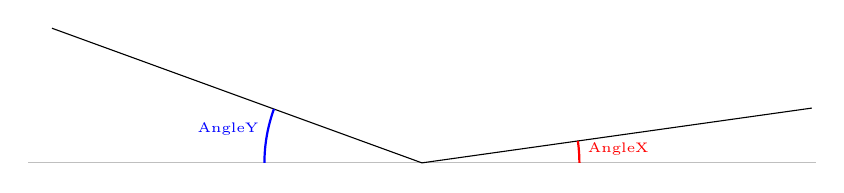
\begin{tikzpicture}
		\draw[lightgray] (-5,0)--(5,0) ;
		\draw[black] (0,0)--++(8:5) ;
		\draw[black] (0,0)--++(160:5) ;
		\draw[thick,red] (2,0) arc (0:8:2) ;
		\draw[red] (4:2.5) node[font=\tiny] {AngleX};
		\draw[thick,blue] (160:2) arc (160:180:2) ;
		\draw[blue] (170:2.5) node[font=\tiny] {AngleY};
	\end{tikzpicture}
\end{center}
\end{tipblock}

\begin{PresCodeTexPL}{}
\xintFor* #1 in {\xintSeq{1}{5}}\do{\ChateauCartes[Legende]{#1}}
\end{PresCodeTexPL}

\begin{PresCodeTexPL}{}
\xintFor* #1 in {\xintSeq{1}{5}}\do{\ChateauCartes[Bas,Legende=false,CouleurDeco=red]{#1}}
\end{PresCodeTexPL}

\begin{PresCodeTexPL}{}
\ChateauCartes[CouleurDeco=teal,Deco=hachures,Echelle=2,Legende]{4}
\end{PresCodeTexPL}

\pagebreak

\section{Allumettes}\label{allumettes}

\subsection{Introduction}

\begin{tipblock}
\cmaj{3.00d} L'idée est de proposer une commande pour représenter des allumettes, créées (et à insérer) dans un environnement \ctex{tikzpicture}.

\smallskip

L'idée est de :

\begin{itemize}
	\item déclarer les points \textit{support} pour le placement des allumettes ;
	\item positionner les allumettes par rapport aux point \textit{support} existants.
\end{itemize}

Le code se charge de placer correctement l'allumette, en fonction de la distance et de l'angle entre les points \textit{support}.

\smallskip

La forme générale de l'allumette est fixée, et les dimensions (internes) sont données en cm.
\end{tipblock}

\begin{PresCodeTexPL}{listing only}
%dans un environnement tikzpicture
\PfLAllumettes[clés]{liste des chemins}
\end{PresCodeTexPL}

\begin{PresCodeTexPL}{}
\begin{tikzpicture}
	\coordinate (A) at (0,0) ; \coordinate (B) at (60:4) ; \coordinate (C) at (4,0) ;
	\filldraw (A) circle[radius=2pt] (B) circle[radius=2pt] (C) circle[radius=2pt] ; %points de contrôle
	\PfLAllumettes{A>B B>C C>A}
\end{tikzpicture}
\end{PresCodeTexPL}

\begin{cautionblock}
Pour cette commande, il est conseillé de ne pas utiliser d'option type \ctex{scale} pour l'environnement \ctex{tikzpicture}, mais plutôt de spécifier les unités en \textit{dur}, via \ctex{x=...,y=...}.
\end{cautionblock}

\subsection{Clés et options}

\begin{cautionblock}
Les \Cle{clés} disponibles pour cette commande sont :

\begin{itemize}
	\item la clé \Cle{CouleurBois} : = couleur du \textit{manche}, et valant \Cle{BoisAllumette} par défaut ;
	\item la clé \Cle{CouleurBout} := couelur du \textit{bout}, et valant \Cle{GratteAllumette} par défaut ;
	\item la clé \Cle{Decal} := espacement par rapport aux point \textit{support}, et valant \Cle{0.224cm} par défaut ;
	\item le booléen \Cle{NoirBlanc} := forcer un affichage N\&B (par défaut \Cle{false}).
\end{itemize}

L'argument obligatoire, entre \ctex{\{...\}}, correspond à la liste des chemins, sous la forme \ctex{A1>B1 A2>B2 ...}.
\end{cautionblock}

\begin{PresCodeTexPL}{}
\begin{tikzpicture}
	\coordinate (A) at (0,0) ; \coordinate (B) at (60:4) ; \coordinate (C) at (4,0) ;
	\PfLAllumettes[CouleurBout=orange,CouleurBois=yellow]{A>B B>C C>A}
\end{tikzpicture}
\end{PresCodeTexPL}

\begin{PresCodeTexPL}{}
\begin{tikzpicture}[x=1.25cm,y=1.25cm]
	\coordinate (A) at (0,0) ; \coordinate (B) at (0,4) ; \coordinate (C) at (4,4) ; \coordinate (D) at (4,0) ;
	\coordinate (E) at ($(B)+(60:4)$) ;
	\PfLAllumettes[Decal=1mm,NoirBlanc]{A>B B>C C>D D>A B>E E>C}
\end{tikzpicture}
\end{PresCodeTexPL}

\pagebreak

\section{Pyramide de sphères}\label{pyramballes}

\subsection{Introduction}

\begin{tipblock}
\cmaj{3.10b} L'idée est de proposer une commande pour représenter, de manière basique, un empilement de sphères.

\smallskip

La visualisation est fixée, mais quelques éléments de personnalisations sont possibles.
\end{tipblock}

\begin{PresCodeTexPL}{listing only}
\EmpilementBalles[clés]{étage(s)}
\end{PresCodeTexPL}

\begin{PresCodeTexPL}{text only}
\EmpilementBalles[clés]{4}
\end{PresCodeTexPL}

\subsection{Clés et options}

\begin{cautionblock}
Les \Cle{clés} disponibles pour cette commande sont :

\begin{itemize}
	\item la clé \Cle{Couleur} := couleur des boules (\Cle{gray} par défaut) ;
	\item la clé \Cle{Echelle} := échelle globale (\Cle{1} par défaut) ;
	\item la clé \Cle{Rotation} := rotation, à manipuler avec précaution (\Cle{-5} par défaut).
\end{itemize}

L'argument obligatoire correspond au nombre d'étages à afficher, sous la forme \ctex{n} ou \ctex{deb-fin}.
\end{cautionblock}

\begin{PresCodeTexPL}{}
\EmpilementBalles{4}%
\EmpilementBalles[Rotation=-10,Couleur=orange]{4}%
\EmpilementBalles[Echelle=0.5]{8}
\end{PresCodeTexPL}

\begin{PresCodeTexPL}{}
\EmpilementBalles[Echelle=0.33,Couleur=red]{3-8}
\end{PresCodeTexPL}

\pagebreak

\section{Commandes pour les dates}\label{dates}

\subsection{Introduction}

\begin{tipblock}
\cmaj{3.10b} L'idée est de proposer, en partenariat avec le package \ctex{datetime2} (qui sera, le cas échéant, chargé avec l'option \ctex{[fr-FR]}) des commandes sur les dates :

\begin{itemize}
	\item afficher le jour (en littéral) correspondant à une date donnée ;
	\item afficher la date complète avec le nom du jour ;
	\item afficher le nombre de jours entre deux dates ;
	\item afficher la date augmentée d'un nombre de jours.
\end{itemize}
\vspace*{-\baselineskip}\leavevmode
\end{tipblock}

\begin{PresCodeTexPL}{listing only}
%version étoilée pour une majuscule au début
\JourSelonDate(*){jj/mm/aaaa}

%version étoilée pour une majuscule au début
\DateComplete(*){jj/mm/aaaa}

%version étoilée pour afficher
%résultat stocké dans \nbjoursentre par défaut
\NbJoursEntreDates(*){jj/mm/aaaa}{jj/mm/aaaa}[\macro]

%version étoilée pour un format jj/mm/aaaa
\AjoutJoursDate(*){jj/mm/aaaa}{nb}
\end{PresCodeTexPL}

\subsection{Exemples}

\begin{PresCodeTexPL}{}
Le 14 mai 1952 était un \JourSelonDate{14/05/1952}.

\JourSelonDate*{04/10/1954} 4 octobre 1954.

\DateComplete*{15/08/1980} est un grand jour pour moi !
\end{PresCodeTexPL}

\begin{PresCodeTexPL}{}
\NbJoursEntreDates{14/05/1952}{15/08/1980}%stockée dans \nbjoursentre
Entre le 14 mai 1952 et le 15 août 1980, il y a \num{\nbjoursentre} jours.
\end{PresCodeTexPL}

\begin{PresCodeTexPL}{}
100 jours après le 04 octobre 2024, nous serons le \AjoutJoursDate{04/10/2024}{100}.

20 jours après le 25 décembre 2025, nous serons le \AjoutJoursDate*{25/12/2025}{20}.
\end{PresCodeTexPL}

\pagebreak


\section{Machines à transformer, en \TikZ}\label{machtransf}

\subsection{Introduction}

\begin{tipblock}
\cmaj{3.00e} L'idée est de \textit{proposer} une commande pour travailler avec une \og machine à transformer \fg.

La figure est réalisée en \TikZ, et quelques éléments de personnalisations sont disponibles, bien que la forme \textit{globale} soit fixée.
\end{tipblock}

\begin{PresCodeTexPL}{listing only}
\MachineTransformer[clés]{e/s}<options tikz>
\end{PresCodeTexPL}

\begin{PresCodeTexPL}{text only}
\MachineTransformer{}
\end{PresCodeTexPL}

\begin{PresCodeTexPL}{}
\MachineTransformer[Bordure,Tableau,Fct=$2x-5$]%
	{3/1,7/9,10/15,1/$-3$,$-4$/$-13$}
\end{PresCodeTexPL}

\begin{PresCodeTexPL}{}
\MachineTransformer[Auto,Formule={-2*X+7},Bordure,Tableau,Fct=$-2x+7$]%
	{3,5,7,-4,0}
\end{PresCodeTexPL}

\subsection{Clés et options}

\begin{cautionblock}
Les \Cle{clés} disponibles pour cette commande sont :

\begin{itemize}
	\item la clé \Cle{Couleur} := couleur de la machine (\Cle{lightgray} par défaut) ;
	\item la clé \Cle{CouleurFct} := couleur de la flèche (\Cle{white} par défaut) ;
	\item le booléen \Cle{Bordure} := afficher une bordure (\Cle{true} par défaut) ;
	\item le booléen \Cle{AffFleche} := afficher la flèche (\Cle{true} par défaut) ;
	\item la clé \Cle{Hauteur} := hauteur de la machine (\Cle{3} par défaut) ;
	\item la clé \Cle{Largeur} := largeur de la machine (\Cle{2} par défaut) ;
	\item la clé \Cle{Offset} := décalage (H) des blocs (\Cle{4pt} par défaut) ;
	\item la clé \Cle{CouleurBloc} := couleur des blocs (\Cle{red} par défaut) ;
	\item le booléen \Cle{Tableau} := afficher le tableau des valeurs (\Cle{false} par défaut) ;
	\item la clé \Cle{PoliceTbl} := police des éléments du tableau (\Cle{\textbackslash footnotesize} par défaut) ;
	\item le booléen \Cle{Logo} := afficher le logo dans la machine (\Cle{true} par défaut) ;
	\item la clé \Cle{Fct} := fonction à afficher (si non vide) ;
	\item le booléen \Cle{Auto} := calcul automatique des images (\Cle{false} par défaut) ;
	\item la clé \Cle{Formule} := formule (variable \ctex{X}) dans le cas \Cle{Auto=true}
	\item le booléen \Cle{ES} := afficher des blocs vides, si pas de tableau (\Cle{false} par défaut) ;
	\item la clé \Cle{Echelle} := modifier l'échelle globale, y compris du texte (\Cle{1} par défaut).
\end{itemize}

L'argument obligatoire, entre \ctex{\{...\}}, correspond à la liste des entrées/sorties :

\begin{itemize}
	\item sous la forme \ctex{x1/y1,x2/y2,...} dans le cas \textit{manuel} (\Cle{Auto=false}) ;
	\item sous la forme \ctex{x1,x2,...} dans le cas \textit{automatique} (\Cle{Auto=true}).
\end{itemize}

\smallskip

À noter que dans le cas \Cle{Auto}, les valeurs sont en mode mathématique, alors qu'en mode \Cle{Auto=false}, il faut le rajouter avec des \ctex{\$...\$}.

\smallskip

L'argument optionnel, et entre \ctex{<...>}, correspond à des options spécifiques, en langage \TikZ, à passer à l'environnement créé.
\end{cautionblock}

\begin{importantblock}
Dans le cas où les calculs seraient faits en automatique :

\begin{itemize}
	\item attention aux valeurs fractionnaires et/ou approchées (pas de gestion de ces cas de figure) ;
	\item l'expression (\Cle{Formule}) de la fonction doit être en langage \ctex{xint}, avec \ctex{X} comme variable !
\end{itemize}
\end{importantblock}

\begin{PresCodeTexPL}{}
\MachineTransformer[Fct=$f$]{$x$/$y$}
\end{PresCodeTexPL}

\begin{PresCodeTexPL}{}
\MachineTransformer[Tableau]{3/1,7/9,10/15,1/$-3$,$-4$/$-13$}
\end{PresCodeTexPL}

\begin{PresCodeTexPL}{}
\MachineTransformer[Bordure,Tableau,Fct=$2x-5$]%
	{3/1,7/9,10/15,1/$-3$,$-4$/$-13$}
\end{PresCodeTexPL}

\begin{PresCodeTexPL}{}
\MachineTransformer[Auto,Formule={-2*X+7},Bordure,Tableau,Fct=$-2x+7$]%
	{3,5,7,-4,0}
\end{PresCodeTexPL}

\begin{PresCodeTexPL}{}
\MachineTransformer[%
	Echelle=1.25,Tableau,Couleur=orange,CouleurFct=teal,%
	CouleurBloc=purple,Offset=1mm
	]%
	{4/5}
\end{PresCodeTexPL}